\section{Modellazione del singolo patch}

\subsection{Dimensionamento del patch con il modello di \emph{Carver}}
Il primo passo verso la progettazione dell'antenna è il dimensionamento del singolo patch, per svolgere questi calcoli, ed anche i successivi, sono stati sviluppati alcuni script in \emph{Python}, ciò ha portato alcuni vantaggi come la possibilità di automatizzare le operazioni e di avere valori teorici molto precisi.
Il primo passo da compiere è la scelta del dielettrico, è stato scelto un \emph{Duroid 5880} (Fig. \ref{img:duroid}), con costante dielettrica $\epsilon_r = 2.2$ e angolo di perdita  $tan \theta = 0.0009$.
\begin{figure}
\centering
\caption{Duroid 5880.}
\label{img:duroid}
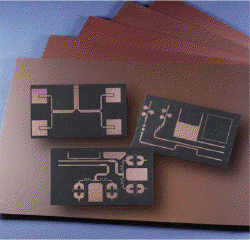
\includegraphics[scale=0.3]{Immagini/duroid}
\end{figure}

Il passo successivo è il calcolo dell'altezza massima del dielettrico che garantisce la
trascurabilità dei modi d'onda superficiali presenti nel patch a causa della discontinuità dielettrica. L'altezza scelta per il substrato dielettrico deve essere inferiore od uguale a questo valore.
\begin{align}
\label{eq:hmax}
h_{max} = \frac{0.3 c}{2 \pi f_{0} \sqrt{\epsilon_{r}}} = 1.66503477015 mm
\end{align}

Si calcola quindi la larghezza del patch:
\begin{align}
\label{eq:w}
W = \frac{c}{2f_0}\sqrt{\frac{2}{\epsilon_r+1}} = 20.4457607338 mm 
\end{align} 

\begin{minted}[linenos=true,frame=leftline,xleftmargin=0.5cm,fontsize=\footnotesize]{python}
# Velocita' della luce [m/s]
c = 3*10**8
# Imedenza del cavo coassiale [Ohm]
r = 50
# Costante dielettrica del Duroid 5880
epsilon_r = 2.2
# Frequenza di risonanza [Hz]
f = 5.8*10**9
# Altezza massima del substrato [mm]
h_max = (0.3*c)/(2*cmath.pi*f*cmath.sqrt(epsilon_r)).real
# Larghezza del patch [mm]
w = (c/(2*f)*cmath.sqrt(2/(epsilon_r+1))).real
\end{minted}

A questo punto è possibile utilizzare $h_{max}$(\ref{eq:hmax}) e $W$(\ref{eq:w}) per ottenere le altre dimensioni del patch. \\
Lo script sviluppato contiene i parametri del \emph{Duroid 5880}, e, inserito un valore per lo spessore $h$ del substrato inferiore a quello calcolato (\ref{eq:hmax}), calcola automaticamente la lunghezza del patch e del punto di alimentazione. \\
\begin{minted}[linenos=true,frame=leftline,xleftmargin=0.5cm,fontsize=\footnotesize]{python}
h = get_h(h_max)
\end{minted}

\begin{minted}[linenos=true,frame=leftline,xleftmargin=0.5cm,fontsize=\footnotesize]{python}
def get_h(h_m):
    while(True):
        h = float(input("introdurre lo spessore del substrato (minore di" + str(h_m*1000)+" mm) \n"))
        if h > 0 and h < h_m*1000:
            return h/1000
\end{minted}
La lunghezza del patch può essere ottenuta mediante la formula successiva:
\begin{align}
L = \frac{c}{2f_0\sqrt{\epsilon_r}} - 2 \Delta L = 16.8984183063 mm 
\end{align}
dove: 
\begin{itemize}
\item Estensione del campo di Fringe :
$\begin{aligned}
\Delta L = 0.412 h \frac{(\epsilon_{eff}+0.3)(\frac{W}{h}+0.264)}{(\epsilon_{eff}-0.258)(\frac{W}{h}+0.8)} 
\end{aligned}$
\item Costante dielettrica efficace:
$\begin{aligned}
\epsilon_{eff} = \frac{\epsilon_r+1}{2} + \frac{\epsilon_r-1}{2} (1 + \frac{h}{W})^{-1}
\end{aligned}$
\item Lunghezza d'onda:
$\begin{aligned}
\lambda = \frac{\lambda_0}{\sqrt{\epsilon_{eff}}}
\end{aligned}$
\end{itemize}

\begin{minted}[linenos=true,frame=leftline,xleftmargin=0.5cm,fontsize=\footnotesize]{python}
lunghezza = getLength(w,h,c,f,epsilon_r)
\end{minted}
\begin{minted}[linenos=true,frame=leftline,xleftmargin=0.5cm,fontsize=\footnotesize]{python}
def getLength(w, h , c , f , epsilon_r):
    # Costante dielettrica efficace
    epsilon_eff = ((epsilon_r+1) + (epsilon_r-1)*(1+12*h/w)**(-0.5))/2
    delta_l = h * 0.412 * ( epsilon_eff + 0.3 )*( w/h + 0.264 )/((epsilon_eff - 0.258 )*( w/h + 0.8 ))
    l = c/( 2 * f * cmath.sqrt(epsilon_eff) ) - 2 * delta_l
    return l.real
\end{minted}

Infine si calcola il punto di alimentazione:
\begin{align}
l_a = \frac{1}{\beta} arccos\biggr(\sqrt{\frac{R_{in}}{R}}\biggr) = 5.32528400943 mm
\end{align}

dove: 
\begin{itemize}
\item Costante di fase:
$\begin{aligned}
\beta = \frac{2 \pi \sqrt{\epsilon_r}}{\lambda_0} 
\end{aligned}$
\item Impedenza d'ingresso desiderata:
$\begin{aligned}
R_{in} = 50 \Omega
\end{aligned}$
\item Resistenza di radiazione:
$\begin{aligned}
R_r = \frac{1}{2G_s} = \frac{60 \lambda_0}{W} \biggr[ 1-\frac{1}{24} \biggr( \frac{2 \pi h}{\lambda_0} \biggr) ^2 \biggr] ^{-1}
\end{aligned}$
\end{itemize}
\begin{minted}[linenos=true,frame=leftline,xleftmargin=0.5cm,fontsize=\footnotesize]{python}
l_alimentazione = getFeedPoint(f , h , w , r , c , epsilon_r )
\end{minted}

\begin{minted}[linenos=true,frame=leftline,xleftmargin=0.5cm,fontsize=\footnotesize]{python}
def getFeedPoint(f , h , w , r , c , epsilon_r):
    lambda_0 = c/f
    r_r = 60*lambda_0/w * (1 - 1/24*(2*cmath.pi*h/lambda_0)**2)**(-1)
    l = lambda_0 / (2*cmath.pi * cmath.sqrt(epsilon_r))*cmath.acos(cmath.sqrt(r/r_r))
    return l.real
\end{minted}

L'output dello script mostrato in frammenti nel paragrafo è un file di testo con tutte le informazioni utili per poter realizzare il singolo patch con \emph{FEKO}.

\begin{minted}[linenos=true,frame=leftline,xleftmargin=0.5cm,fontsize=\footnotesize]{python}
h = 1.0 mm 
la = 5.32528400943 mm 
W = 20.4457607338 mm 
h_max = 1.66503477015 mm 
L = 16.8984183063 mm 
\end{minted}

\subsection{Creazione del modello del patch con FEKO}
\subsubsection*{Modello teorico}
Una volta ottenute le dimensioni del patch è possibile realizzarne un modello tridimensionale attraverso l'uso del CAD elettrmagnetico \emph{FEKO}, nella figura \ref{img:patch} è mostrato il patch realizzato.
\begin{figure}
\centering
\caption{Patch realizzato in FEKO con le relative dimensioni.}
\label{img:patch}
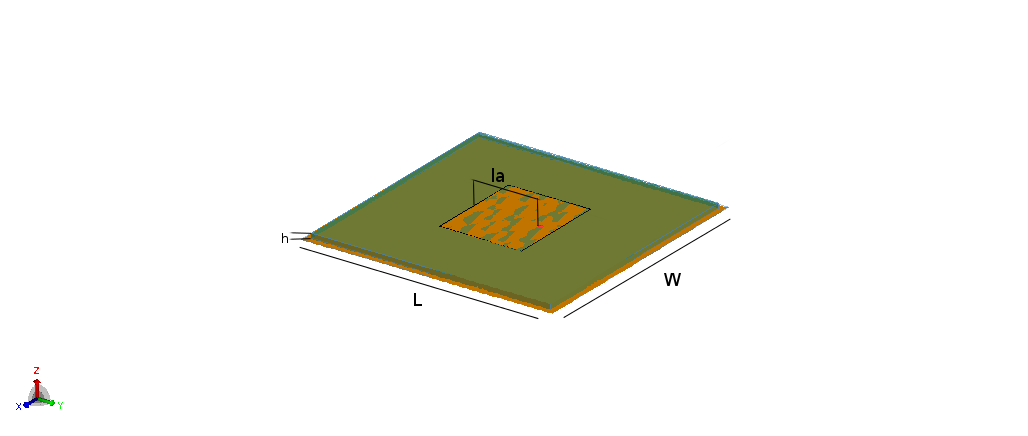
\includegraphics[scale=0.5]{Immagini/patch_original_dim}
\end{figure}

Con l'utilizzo di \emph{POSTFEKO} è possibile rielaborare i dati precedenti per ottenere informazioni riguardo al patch, si è scelto di rappresentare il coefficiente di riflessione e l'impedenza di ingresso. \\
Nella figura \ref{img:reflori} è mostrata l'attenuazione del coefficiente di riflessione, come evidenziato nella figura, si può notare che c'è un minimo in $5.81167 GHz$ a $-8.83847 dB$, inoltre alla frequenza di risonanza $f_0 = 5.8 GHz$ l'attenuazione è di $-8.82411 dB$. \\
I valori conseguiti non rispettano le specifiche di progetto, inoltre non è neanche possibile calcolare la banda percentuale a $-15 dB$.
\begin{figure}
\centering
\caption{Coefficiente di riflessione relativo alla configurazione teorica del patch.}
\label{img:reflori}
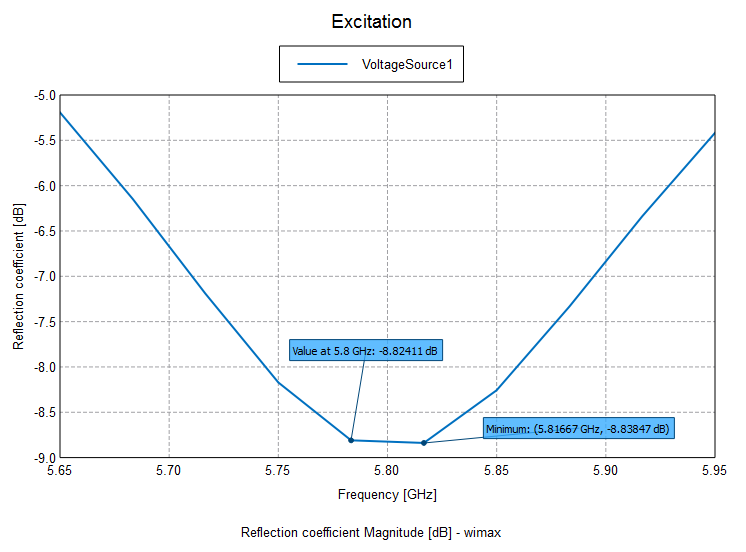
\includegraphics[scale=0.5]{Immagini/reflection_coefficient_original}
\end{figure}

La figura \ref{img:impori} mostra i valori dell'impedenza d'ingresso alla frequenza di risonanza: la parte reale dell'impedenza è di $\Re{[Z]} = 51.1 \Omega $, la parte immaginaria è di  $\Im{[Z]} = -38.3 \Omega$. La parte reale andrebbe bene ma la parte immaginaria ad un valore così alto porterebbe a ingenti perdite di potenza.

\begin{figure}
\centering
\caption{Parte reale e parte immaginaria dell'impedenza relative alla configurazione teorica del patch.}
\label{img:impori}
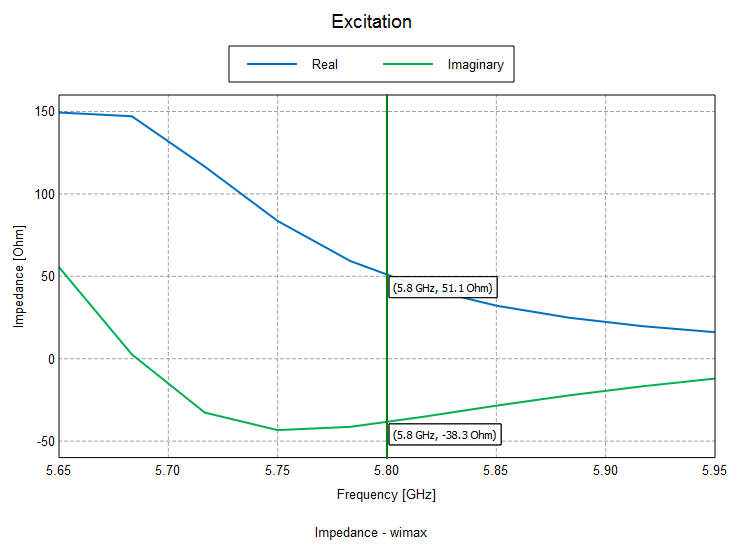
\includegraphics[scale=0.5]{Immagini/impedance_original}
\end{figure}

\subsubsection*{Ottimizzazione del modello teorico}
I risultati ottenuti con i modelli teorici mostrano come non solo non siano soddisfatte le specifiche di progetto ma anche come, volendo utilizzare tale modello, si ottengano bassissime prestazioni. \\
Per ottimizzare il modello teorico è necessario variare i valori dati in input a \emph{POSTFEKO}: le dimensioni del patch. Riuscendo quindi a cambiare opportunamente $W$, $L$, $la$ e $h$ è possibile adempiere alle specifiche di progetto, le quali riferendosi al momento al singolo patch, si traducono nell'ottenere un'\emph{attenuazione del coefficiente di riflessione inferiore a 15 dB}, portare la \emph{parte reale dell'impedenza di ingresso ad un valore prossimo allo zero} e nell'avere \emph{una banda percentuale superiore al 2\%}. \\
La realizzazione di ognuna delle specifiche non è indipendente l'una dall'altra, spesso, infatti, il soddisfacimento di una specifica porta al peggioramento di un'altra. Quindi anche la variazione di alcune dimensioni del patch porta a variazioni, anche molto diverse, dei tre obiettivi da raggiungere. \\
Dopo numerose prove, sono stati scelte le seguenti dimensioni (tabella \ref{tab:confronto}) che porteranno ai risultati mostrati nelle figure \ref{img:reflopt}, \ref{img:impopt}, \ref{img:polar}.

\begin{table}[h]\footnotesize
\caption{Confronto tra i valori teorici e quelli ottimizzati.}
\label{tab:confronto}
\begin{tabularx}{\textwidth}{XXXXXX}
\toprule
Valori & $h(m)$ & $L(m)$ & $l_a(m)$ & $W(m)$ \\
\midrule
Teorici & 1 & 16.8984183063 & 5.32528400943 & 20.4457607338 \\
Ottimizzati & 1.6 & 16.5 & 4.3 & 20.5 \\
\bottomrule
\end{tabularx}
\end{table}
  
La figura \ref{img:reflopt} mostra i valori dell'attenuazione del coefficiente di riflessione, si ha un minimo alla frequenza di $5.78 GHz$ pari a $-36.01 dB$, alla frequenza di risonanza, invece, si ha un valora inferiore, $-28.2  dB$, che comunque soddisfa le specifiche di progetto. \\
Altro dato molto importante è il soddisfacimento del requisito sulla banda percentuale, nella figura è evidenziata la banda a $-15 dB$, $0.123535 GHz$. La banda percentuale si ottiene dalla formula:
\begin{align}
B_{\%} = \frac{\Delta f}{f_0} = 2.13\%
\end{align}
Il valore supera di $0.13\%$ quello richiesto. \\[1cm]

\begin{figure}
\centering
\caption{Coefficiente di riflessione adattato alle specifiche di progetto.}
\label{img:reflopt}
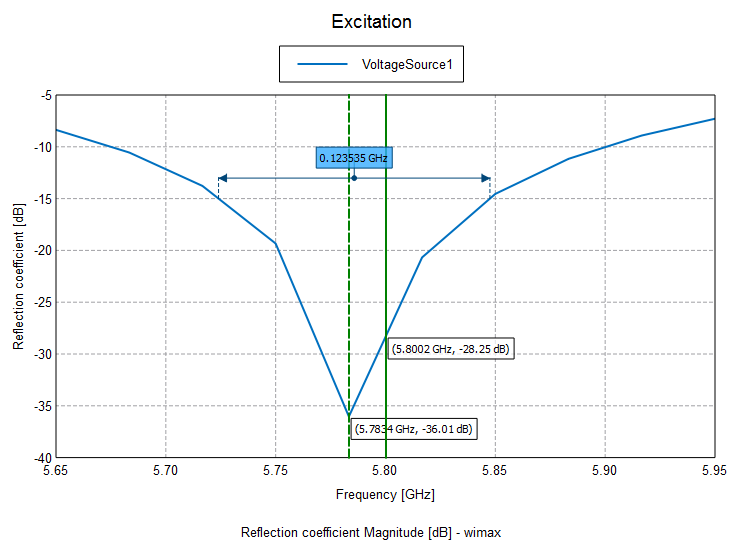
\includegraphics[scale=0.5]{Immagini/reflection_coefficient_optimized}
\end{figure}

Nella figura \ref{img:impopt} sono rappresentati i valori della parte reale e della parte immaginaria dell'impedenza di ingresso, un confronto con i valori precedenti mostra come la parte reale sia di poco inferiore alla precedente $46.1 \Omega$ ma la parte immaginaria sia prossima allo zero $-0.726 \Omega$; molto importante è quest'ultimo valore, dimostra come siano quasi nulle le perdite di potenza dovute all'impedenza d'ingresso. \\[1cm]

\begin{figure}
\centering
\caption{Parte reale e parte immaginaria dell'impedenza adattate alle specifiche di progetto.}
\label{img:impopt}
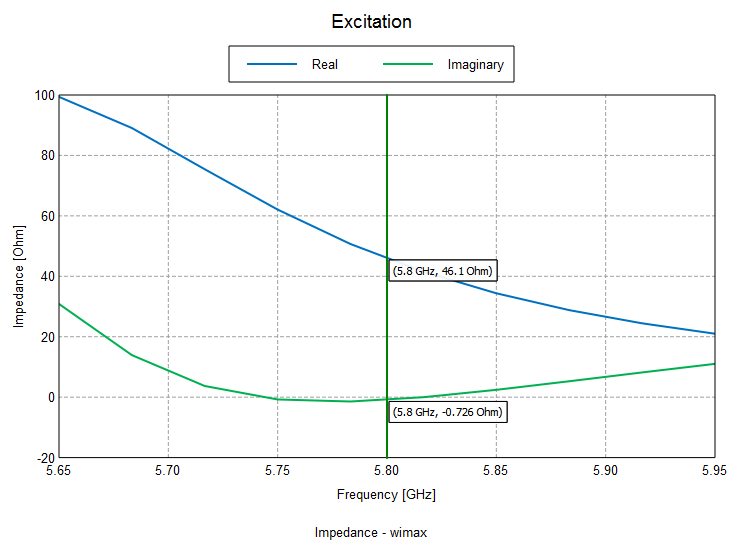
\includegraphics[scale=0.5]{Immagini/impedance_optimized}
\end{figure}

La figura \ref{img:polar}, infine, mostra il diagramma polare del guadagno in dB, sul taglio $E(\phi=\frac{\pi}{2})$ nella direzione di \emph{broadside}, $\theta = \frac{\pi}{2}$. Il guadagno è pari a $7.26 dB$.

\begin{figure}
\centering
\caption{Diagramma polare del guadagno in scala logaritmica.}
\label{img:polar}
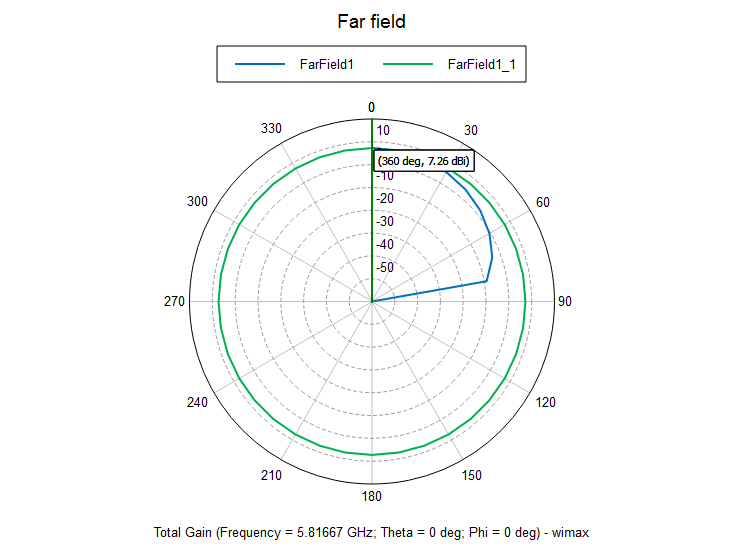
\includegraphics[scale=0.5]{Immagini/total_gain_optimized}
\end{figure}